\documentclass[aspectratio=169,14pt]{beamer}

% ── KuliBayar Theme ──────────────────────────────────────────────
\usepackage[utf8]{inputenc}
\usepackage{graphicx}
\usepackage{fontspec}
\usepackage{tikz}
\usepackage{hyperref}
\usepackage{qrcode}
\usepackage{microtype}

\usetikzlibrary{shapes.geometric, arrows, positioning, calc}

% Colors
\definecolor{kgray}{HTML}{050505}
\definecolor{kwhite}{HTML}{E5E5E5}
\definecolor{korange}{HTML}{FF4500}
\definecolor{kmuted}{HTML}{A0A0A0}
\definecolor{kdark}{HTML}{171717}

% Beamer overrides
\setbeamercolor{background canvas}{bg=kgray}
\setbeamercolor{normal text}{fg=kwhite}
\setbeamercolor{title}{fg=kwhite}
\setbeamercolor{subtitle}{fg=kmuted}
\setbeamercolor{frametitle}{fg=kwhite}
\setbeamercolor{itemize item}{fg=korange}
\setbeamercolor{itemize subitem}{fg=kmuted}
\setbeamercolor{enumerate item}{fg=korange}
\setbeamerfont{frametitle}{size=\LARGE, series=\bfseries}
\setbeamertemplate{navigation symbols}{}
\setbeamertemplate{itemize items}[circle]

% Tighter spacing for itemize
\setlength{\leftmargini}{1.2em}
\setlength{\itemsep}{0.3em}
\setlength{\parskip}{0pt}

% Frame title bar
\setbeamertemplate{frametitle}{
  \vspace{0.3em}
  \usebeamerfont{frametitle}\insertframetitle\par
  \vspace{0.2em}
  \textcolor{korange}{\rule{\textwidth}{0.5pt}}
}

% ── Custom macros ────────────────────────────────────────────────
\newcommand{\highlight}[1]{\textcolor{korange}{\textbf{#1}}}
\newcommand{\stat}[2]{\begin{minipage}{0.3\textwidth}\centering\textcolor{korange}{\Huge\bfseries#1}\\\textcolor{kmuted}{\small #2}\end{minipage}}

% ── Title page ───────────────────────────────────────────────────
\title{KuliBayar}
\subtitle{\textcolor{korange}{Bayaran Kuli, Dijamin On-Chain}}
\date{Indonesia Web3 Hackathon 2026 \\ \vspace{0.3em} \textcolor{kmuted}{\small Finance \& Commerce Track}}

\begin{document}

% ── Slide 0: Title ──────────────────────────────────────────────
\begin{frame}[plain]
\vfill
\begin{center}
  {\fontsize{48}{56}\selectfont\textcolor{kwhite}{KuliBayar}}\\[0.3em]
  {\fontsize{18}{24}\selectfont\textcolor{korange}{Bayaran Kuli, Dijamin On-Chain}}\\[2em]
  {\small\textcolor{kmuted}{Indonesia Web3 Hackathon 2026 — Finance \& Commerce Track}}\\[0.5em]
  {\small\textcolor{kmuted}{Tim JAW}}
\end{center}
\vfill
\end{frame}

% ── Slide 1: Problem ────────────────────────────────────────────
\begin{frame}{Masalah}
\begin{itemize}
  \item \highlight{8,7 juta} pekerja konstruksi di Indonesia (BPS 2025)
  \item \highlight{59\%} pekerja Indonesia berada di sektor informal — tanpa kontrak, tanpa jaminan
  \item \highlight{32\%} proyek konstruksi alami keterlambatan pembayaran $>$60 hari
  \item Sengketa kerja selalu \highlight{merugikan kuli} — tidak ada bukti on-chain
\end{itemize}

\vspace{0.8em}
\begin{center}
\stat{8,7 Juta}{Pekerja Konstruksi} \hfill \stat{1 dari 3}{Proyek Telat Bayar} \hfill \stat{Rp 0}{Jaminan Kontrak}
\end{center}
\end{frame}

% ── Slide 2: Solution ───────────────────────────────────────────
\begin{frame}{Solusi}
\small
\begin{columns}[T]
\column{0.5\textwidth}
  \textbf{Platform escrow on-chain} yang:
  \begin{itemize}
    \item Mengunci dana kontraktor di \highlight{smart contract}
    \item Membayar kuli harian setelah kerja \highlight{terverifikasi} via foto + GPS
    \item Membangun \highlight{reputasi on-chain} yang tidak bisa dihapus
  \end{itemize}

\column{0.5\textwidth}
  \begin{center}
  \fcolorbox{korange}{kdark}{\parbox{0.85\textwidth}{\centering
    \textcolor{korange}{\textbf{Mengapa Escrow?}}\\[0.3em]
    \textcolor{kwhite}{Dana tidak bisa dicairkan sepihak.}\\
    \textcolor{kwhite}{Kuli dibayar otomatis setelah bukti kerja.}\\
    \textcolor{kwhite}{Kontraktor tidak perlu khawatir uang hilang.}
  }}
  \end{center}
\end{columns}
\end{frame}

% ── Slide 3: How It Works ───────────────────────────────────────
\begin{frame}{Cara Kerja}
\sloppy
\begin{center}
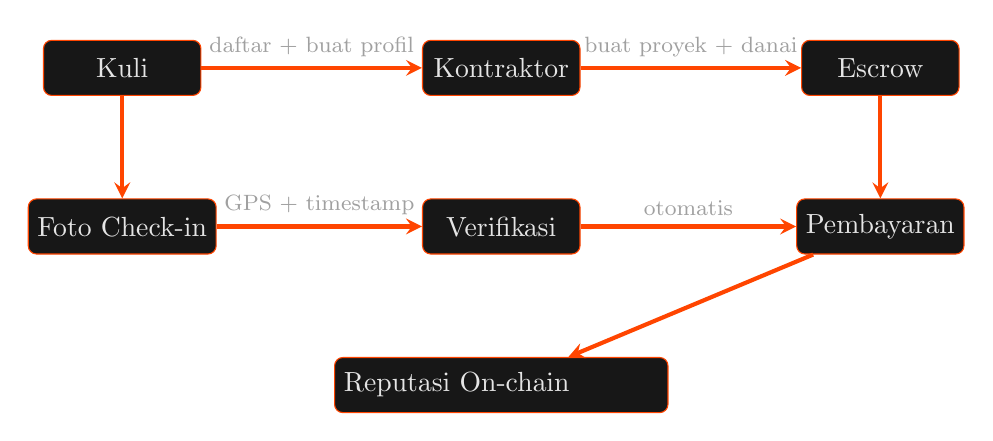
\begin{tikzpicture}[node distance=0.7cm]

\tikzstyle{box} = [rectangle, draw=korange, fill=kdark, text=kwhite, minimum width=2cm, minimum height=0.7cm, rounded corners=3pt]
\tikzstyle{arrow} = [->, >=stealth, korange, line width=1.5pt]
\tikzstyle{label} = [text=kmuted, font=\footnotesize]

% Row 1
\node[box] (kuli) {Kuli};
\node[box, right=2.8cm of kuli] (kontraktor) {Kontraktor};
\node[box, right=2.8cm of kontraktor] (escrow) {Escrow};

\draw[arrow] (kuli) -- node[label, above]{daftar + buat profil} (kontraktor);
\draw[arrow] (kontraktor) -- node[label, above]{buat proyek + danai} (escrow);

% Row 2
\node[box, below=1.3cm of kuli] (foto) {Foto Check-in};
\node[box, below=1.3cm of kontraktor] (verif) {Verifikasi};
\node[box, below=1.3cm of escrow] (bayar) {Pembayaran};

\draw[arrow] (escrow) -- (bayar);
\draw[arrow] (kuli) -- (foto);
\draw[arrow] (foto) -- node[label, above]{GPS + timestamp} (verif);
\draw[arrow] (verif) -- node[label, above]{otomatis} (bayar);

% Reputation
\node[box, below=1.3cm of verif, text width=4cm] (rep) {Reputasi On-chain};
\draw[arrow] (bayar) -- (rep);

\end{tikzpicture}
\end{center}
\end{frame}

% ── Slide 4: Product Demo ───────────────────────────────────────
\begin{frame}{Demo}
\vspace{0.3em}
\begin{center}
{\large\textcolor{kwhite}{\textbf{KuliBayar Live}}}\\[0.3em]
\fcolorbox{korange}{kdark}{\parbox{0.55\textwidth}{\centering
  \vspace{0.2em}
  \href{https://kulibayar.wedjaw.my.id}{\textcolor{korange}{\normalsize\textbf{kulibayar.wedjaw.my.id}}}\\[0.2em]
  \textcolor{kmuted}{\footnotesize Frontend sudah live — connect MetaMask untuk mencoba}\\[0.2em]
  \qrcode[height=1.5cm]{https://kulibayar.wedjaw.my.id}\\[0.2em]
  \textcolor{kmuted}{\footnotesize Scan QR untuk buka demo}
  \vspace{0.2em}
}}
\end{center}
\end{frame}

% ── Slide 5: Why Blockchain ─────────────────────────────────────
\begin{frame}{Mengapa Blockchain?}
\footnotesize
\begin{columns}[T]
\column{0.5\textwidth}
  \highlight{Trustless}
  \begin{itemize}
    \item Dana tidak bisa digelapkan
    \item Pembayaran otomatis via smart contract
    \item Tidak perlu pihak ketiga
  \end{itemize}

  \vspace{0.2em}
  \highlight{Immutable}
  \begin{itemize}
    \item Reputasi tidak bisa dihapus
    \item Riwayat kerja transparan
    \item Audit trail lengkap
  \end{itemize}

\column{0.5\textwidth}
  \highlight{Cheap \& Fast}
  \begin{itemize}
    \item Polygon Amoy: biaya gas < \$0.001
    \item Finalitas transaksi < 2 detik
    \item Tanpa perantara bank
  \end{itemize}

  \vspace{0.2em}
  \highlight{Inclusive}
  \begin{itemize}
    \item Cukup smartphone + MetaMask
    \item Tidak perlu rekening bank
    \item Bisa diakses oleh 10M+ kuli
  \end{itemize}
\end{columns}
\end{frame}

% ── Slide 6: Market ─────────────────────────────────────────────
\begin{frame}{Market}

\vspace{0.5em}
\begin{itemize}
  \item \highlight{8,7 juta} tenaga kerja konstruksi di Indonesia (\textcolor{kmuted}{\scriptsize BPS 2025})
  \item Sektor konstruksi = \highlight{10,43\%} PDB Indonesia — setara \highlight{Rp2.310 T}
  \item \highlight{35\%} kontraktor alami keterlambatan pembayaran $>$60 hari (\textcolor{kmuted}{\scriptsize Bisnis Indonesia})
  \item \highlight{0} platform escrow khusus konstruksi di Indonesia
\end{itemize}

\vspace{0.8em}
\begin{center}
\fcolorbox{korange}{kdark}{\parbox{0.7\textwidth}{\centering
  \textcolor{korange}{\normalsize\textbf{Potensi Pasar:}}\\
  \textcolor{kwhite}{1\% volume upah konstruksi $\times$ 1\% fee}\\
  \textcolor{kwhite}{= \highlight{Rp23 M++} revenue tahunan}}
\end{center}
\end{frame}

% ── Slide 7: Team ───────────────────────────────────────────────
\begin{frame}{Tim}

\begin{center}
\vspace{1em}
\textcolor{korange}{\LARGE\textbf{Fatih Jawwad}}\\[0.3em]
\textcolor{kmuted}{\large Edge ML \& Rust Engineer}\\[0.5em]
\textcolor{kmuted}{Forum DA'I, UNIDA Gontor}\\[0.5em]
\textcolor{kmuted}{\small 8 PR merged di Burn (Rust ML framework)}\\[0.2em]
\textcolor{kmuted}{\small \mbox{Pengalaman:} Erasmus+ Sevilla, Google Student Ambassador}
\end{center}

\vspace{2em}
\begin{center}
\fcolorbox{korange}{kdark}{\parbox{0.85\textwidth}{\centering
  \textcolor{kmuted}{\small Tech Stack: Solidity $\cdot$ Next.js $\cdot$ Express.js $\cdot$ Polygon Amoy}\\[0.2em]
  \textcolor{kmuted}{\small \href{https://github.com/jaweed3/KuliBayar}{\textcolor{korange}{GitHub}} \qquad $\cdot$ \qquad kulibayar.wedjaw.my.id}
}}
\end{center}
\end{frame}

% ── Slide 8: Ask ────────────────────────────────────────────────
\begin{frame}{Rencana ke Depan}
\small
\begin{itemize}
  \item \highlight{Q3 2026}: Deploy mainnet + Launch MVP di Jabodetabek
  \item \highlight{Q4 2026}: Integrasi WhatsApp bot untuk kuli tanpa smartphone
  \item \highlight{Q1 2027}: AI photo verification (auto-detect selesai)
  \item \highlight{Q2 2027}: Ekspansi ke sektor lain (tani, pabrik, jasa)
\end{itemize}

\vspace{0.5em}
\begin{center}
\fcolorbox{korange}{kdark}{\parbox{0.7\textwidth}{\centering
  \vspace{0.2em}
  \textcolor{korange}{\textbf{Dukungan yang Dibutuhkan}}\\[0.2em]
  \textcolor{kwhite}{• Bimbingan teknis smart contract security}\\
  \textcolor{kwhite}{• Koneksi ke kontraktor untuk pilot project}\\
  \textcolor{kwhite}{• Grant/dev tooling dari ecosystem partner}\\[0.2em]
  \vspace{0.1em}
}}
\end{center}
\end{frame}

% ── Slide 9: Thank You ──────────────────────────────────────────
\begin{frame}[plain]
\vfill
\begin{center}
  {\fontsize{36}{44}\selectfont\textcolor{kwhite}{Terima Kasih}}\\[0.3em]
  {\large\textcolor{korange}{kulibayar.wedjaw.my.id}}\\[1em]
  \textcolor{kmuted}{\small Tim JAW $\cdot$ Indonesia Web3 Hackathon 2026}
\end{center}
\vfill
\end{frame}

\end{document}
